\documentclass{article}
\usepackage[utf8]{inputenc}

\title{Simulation Results (Week-2)}
\date{29 January, 2020}

\usepackage{natbib}
\usepackage{graphicx}
\usepackage[section]{placeins}
\usepackage{amsmath}
\begin{document}

\maketitle

\section{Team details}
{\begin{itemize}
    \item Shaik Mastan Vali - EE18BTECH11039
    \item Dasari Shree Ujjwal - EE18BTECH11010
\end{itemize}}

\section{4-QAM simulation}
{\begin{itemize}
    \item \textbf{Original Image}:
    \begin{figure}[h]
    \centering
    \includegraphics[scale = 0.7]{original_img.jpg}
    \end{figure}
    
    \item \textbf{BER values for different values of \(E_b/N_0\)}: \newline
    Note that the values of the bit error rate and \(Q(\sqrt{2\frac{E_b}{N_0}})\) are approximately equal and the BER decreases with an increase in \(\frac{E_b}{N_0}\).
    \begin{figure}[!htb]
    \centering
    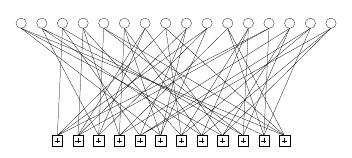
\includegraphics[scale = 0.36]{1.png}
    \end{figure}
    
    \item \textbf{Plot of BER v/s \(\frac{E_b}{N_0}\)}
    \begin{figure}[!htb]
    \centering
    \includegraphics[scale = 0.7]{BER.jpg}
    \end{figure}
\end{itemize}
}
 
\section{Demodulated Images}
{   
    \begin{figure}[h]
    \centering
    \includegraphics[scale = 0.7]{demod_img_EbN0=-10dB.jpg}
    \caption{Demodulated image for \(E_b/N_0 = -10\; dB\)}
    \end{figure}
    
     \begin{figure}[!htb]
    \centering
    \includegraphics[scale = 0.7]{demod_img_EbN0=-5dB.jpg}
    \caption{Demodulated image for \(E_b/N_0 = -5\;dB\)}
    \end{figure}
    
     \begin{figure}[!htb]
    \centering
    \includegraphics[scale = 0.7]{demod_img_EbN0=0dB.jpg}
    \caption{Demodulated image for \(E_b/N_0 = 0\;dB\)}
    \end{figure}
    
     \begin{figure}[!htb]
    \centering
    \includegraphics[scale = 0.7]{demod_img_EbN0=5dB.jpg}
    \caption{Demodulated image for \(E_b/N_0 = 5\;dB\)}
    \end{figure}
}

\section{Explanation of the code}
{
    This section is about the significant variables used in the program.\newline
    \begin{itemize}
        \item \sffamily{img - }\textrm{The matrix which is used to store the pixel values.}
        \item \sffamily{s - }\textrm{The vector which is used to store the signal values generated for the image bits.}
        \item \sffamily{S\_space - }\textrm{The vector which is used to store the unique M-QAM symbols.}
        \item \sffamily{bit\_array - }\textrm{The vector which is used to store the bits corresponding to the symbols in} \sffamily{S\_space}\textrm{. This vector is used in the demodulation scheme later in the program.}
        \item \sffamily{Eb\_N0\_dB - }\textrm{The list which is used to store the given values of \(\frac{E_b}{N_0}\) in dB}.
        \item \sffamily{Eb\_N0 - }\textrm{The list which is used to store the given values of \(\frac{E_b}{N_0}\) in the decimal scale.}
        \item \sffamily{w - }\textrm{The vector which is used to store the AWGN of \(\mu = 0\) and \(\sigma^2 = f_s\frac{N_0}{2}\).}
        \item \sffamily{r\_sym - }\textrm{The vector which is used to store the signal space co-ordinates of }\sffamily{r}.
        \item \sffamily{dist - }\textrm{The vector which is used to store the distance of the signal space co-ordinates from the received vector. These distances are used to find the minimum distance required for demodulation.}
        \item \sffamily{demod - }\textrm{The vector which is used to store the demodulated bits based on the minimum values in} \sffamily{dist}.
        
    \end{itemize}
    
    In the attached program, the signal is modulated according to the given instructions. The 'M' signal space co-ordinates are stored in a vector, which will be used for demodulation. Upon integrating (manually), we get energy of each signal as T, which means \(E_b = \frac{T}{2}\). The given \(\frac{E_b}{N_0}\) values are converted from dB to decimal scale and the corresponding \(N_0\) is generated. With this given value of \(N_0\), the AWGN values are generated and added to \sffamily{s}. 
    
    \textrm{For demodulation scheme, the received signal is represented as signal space co-ordinates. The distance between }\sffamily{r}\textrm{ and the M-QAM symbols are computed. The QAM symbol which gives the minimum distance is stored and the corresponding bit values (two bits) are stored in the }\sffamily{demod }\textrm{vector.}
}

\end{document}
